\section{Conversores}


Uma máquina de corrente contínua pode funcionar tanto como um gerador, convertendo energia mecânica em energia elétrica, quanto como um motor, convertendo energia elétrica em mecânica. Apesar de a energia elétrica ser comumente distribuída (no nível do consumidor) em corrente alternada, os motores de corrente contínua possuem grande participação na indústrias, uma vez que permitem facilmente a variação de velocidade, por exemplo, de uma esteira ou um comboio. 

Por outro lado, componentes eletrônicos de tensão alternada, cada vez mais acessíveis, são capazes de controlar a velocidade de motores assíncronos da mesma forma, logo, pelo seu melhor custo benefício, eles vêm substituindo os motores de corrente contínua na maior parte das aplicações. De toda forma, o estudo dos motores de corrente contínua é fundamental pois introduz os conceitos básicos do funcionamento de máquinas elétricas. A figura \ref{fig:MCC} mostra esquematicamente uma máquina de corrente contínua elementar.

\begin{figure}[ht!]
\center
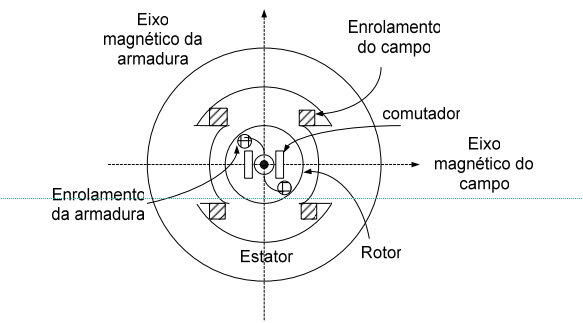
\includegraphics[scale=0.66]{imagens/maquina_cc.png}
\caption{\label{fig:MCC}Máquina de corrente contínua elementar.}
\caption*{Fonte: Máquinas de corrente contínua \protect\footnotemark}
\end{figure}

\footnotetext{Disponível em: <http://www.gsep.ene.unb.br/osem/ivan/Conversao> Acesso em out. 2018.}



\subsection{Conversores CC-CC}

Conversores CC-CC controlam o fluxo de potência entre a entrada e a saída através do chaveamento de semicondutores de potência, i.e., atuando como um interruptor entre a fonte e a carga. Uma ilustração dessa operação pode ser vista na figura \ref{g0cc}, junto do comportamento da tensão sobre a carga.

\begin{figure}[h]
\center
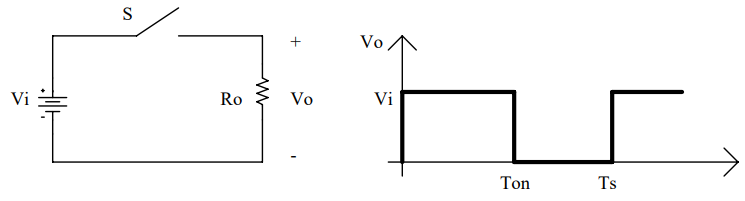
\includegraphics[scale=0.55]{imagens/coversor_cc_circuito_grafico.png}
\caption{Circuito ilustrativo e forma de onda da tensão sobre a carga de um conversor CC-CC.}\label{g0cc}  
\caption*{Fonte: Introdução aos conversores CC-CC (2001)}
\end{figure}

Nesse cenário, denotamos o intervalo de comutação por \[
    T_{s} = \frac{1}{F_{s}}
,\] onde $F_{s}$ representa a frequência de comutação.

Uma forma de mensurar a entrega de tensão à carga é através da razão cíclica \[
    D = \frac{T_{on}}{T_{s}}
,\] onde $T_{on}$ representa o intervalo de condução.

A tensão média pode ser determinada por
\begin{align*}
    V_{o} &= \frac{1}{T_{s}}\int_{o}^{T_{on}}V_{i}dt \\
    &= \frac{T_{on}}{T_{s}}V_{i}\\
    &= D V_i
.\end{align*}

A partir disso, elucida-se o ganho estático do conversor, que é definido como a razão entre a tensão de saída e a tensão de entrada através da razão cíclica, uma vez que \[
D = \frac{V_o}{V_i}
.\]

Pode-se gerar ondas com frequência fixa através da modulação por largura de pulso (\emph{PWM}). A figura \ref{gcp} ilustra uma forma de gerar tal sinal através de um gerador de rampa.

\begin{figure}[h]
\center
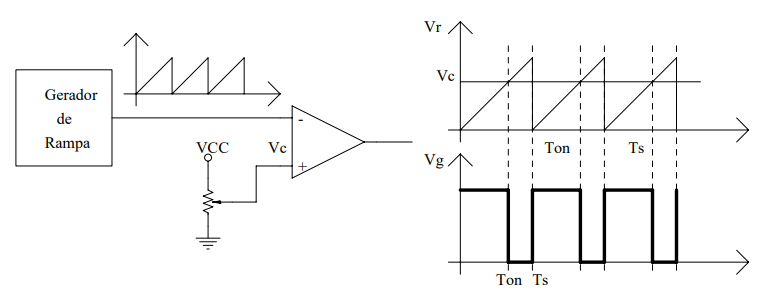
\includegraphics[scale=0.55]{imagens/grafico_circuito_pwm.png}
\caption{Exemplo de um circuito que realiza modulação por largura de pulso.}\label{gcp} 
\caption*{Fonte: Introdução aos conversores CC-CC (2001)}
\end{figure}

Conversores CC-CC são amplamente utilizados em sistemas de alimentação de componentes eletrônicos, principalmente quando não se tem uma preocupação grande com o nível de ruído (harmônicas) do sinal. São componentes amplamente utilizados em fontes chaveadas, alternativas modernas as fontes lineares. Além disso, são de grande uso nos sistemas geradores de energias renováveis e no carregamento de baterias.

\subsubsection{Conversores Buck}


Também conhecido como abaixador de tensão, a principal característica dos conversores buck é o controle da corrente na saída, conforme ilustra a figura \ref{cb}.

\begin{figure}[h]
\center
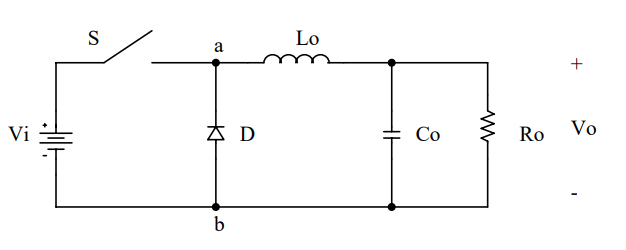
\includegraphics[scale=0.55]{imagens/circuito_buck.png}
\caption{Estrutura do conversor Buck.}\label{cb} 
\caption*{Fonte: Introdução aos conversores CC-CC (2001)}
\end{figure}
 
O seu funcionamento pode ser  descrito em duas etapas. Primeiro, com a chave $S$ em condução, i.e., no período $D \cdot T_s$, a fonte $V_i$ energiza o circuito RLC. No momento em que a chave $S$ abre, no período $\left( 1-D \right) T_s$, o circuito garante inércia da corrente sobre a saída.

Sabendo que a tensão média sobre o atuador, idealmente, é nula, podemos determinar 
\begin{align*}
    V_{o} &= V_{ab,med} =  \frac{1}{T_{s}}\int_{o}^{DT_{s}}V_{i}dt\\
	  &\implies \frac{V_{o}}{V_{i}} = D
.\end{align*} Ou seja, novamente temos uma relação linear entre a razão cíclica e o ganho estático.

A figura \ref{g3b} ilustra o comportamento da tensão e da corrente nos diversos componentes da carga do conversor buck.

\begin{figure}[h]
\center
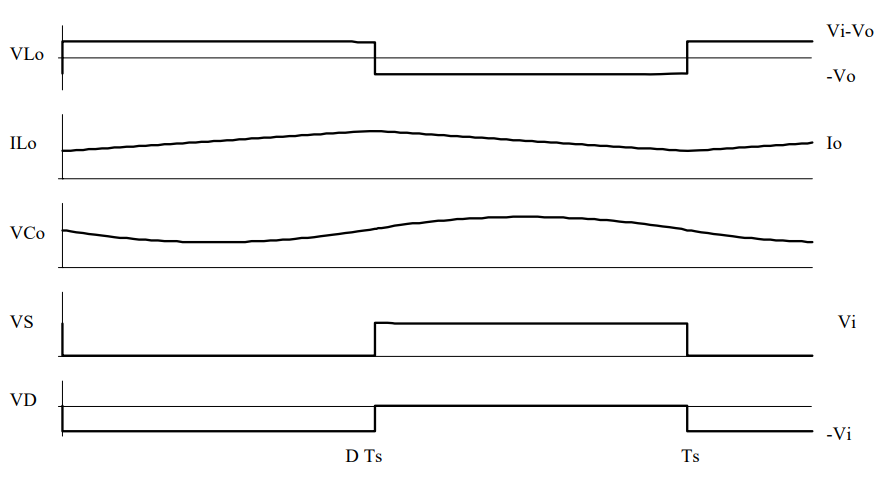
\includegraphics[scale=0.55]{imagens/grafico3_buck.png}
\caption{Formas de onda do conversor Buck.}\label{g3b} 
\caption*{Fonte: Introdução aos conversores CC-CC (2001)}
\end{figure}

De forma similar ao que foi visto nos retificadores, o conversor buck também pode operar em condução contínua, descontínua ou crítica, quando encontra-se na iminência de trocar seu modo de operação.

De modo geral, o conversor Buck está limitado à magnitude da tensão da entrada, mas não tem grande impacto sobre a corrente da saída, i.e., não a distorce muito, ainda que chaveie sempre a corrente fornecida pela alimentação.


 
\subsubsection{Conversores Boost}

O maior diferencial do conversor Boost é a capacidade de elevar a tensão a partir da corrente na entrada. A figura \ref{cboost} ilustra o circuito simplificado de um conversor Boost.

\begin{figure}[h]
\center
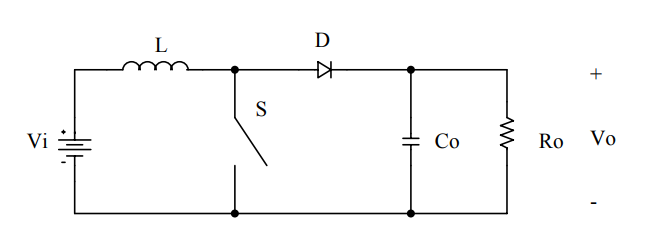
\includegraphics[scale=0.55]{imagens/circuito_boost.png}
\caption{Circuito simplificado do conversor Boost.}\label{cboost} 
\caption*{Fonte: Introdução aos conversores CC-CC (2001)}
\end{figure}

Durante a etapa de condução, com a chave $S$ fechada, o indutor $L$ é magnetizado pela alimentação. Nota-se que a chave age como um curto para a saída, que só é alimentada pelo capacitor $C_o$ uma vez que há o diodo $D$ impedindo que esse seja curto-circuitado pela chave. Quando a chave abre, o indutor e a fonte fornecem energia à saída e ao capacitor, dessa forma, elevando a tensão aparente na saída. O comportamento da tensão no indutor pode ser visto, de forma simplificada, na figura \ref{g1bo}.

\begin{figure}[h]
\center
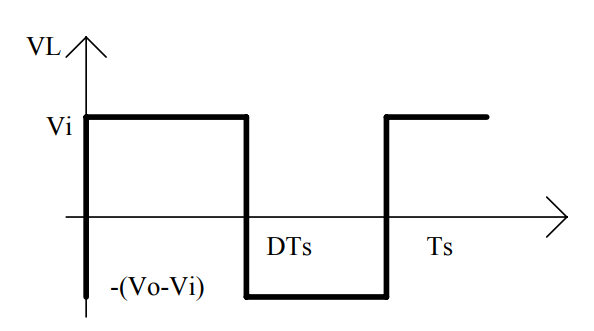
\includegraphics[scale=0.55]{imagens/grafico1_boost.png}
\caption{Comportamento da tensão no indutor de um conversor Boost.}\label{g1bo} 
\caption*{Fonte: Introdução aos conversores CC-CC (2001)}
\end{figure}

Assumindo, com idealidades, que a tensão média sobre o indutor é nula, temos \[
V_o = \frac{1}{T_{s}}\int_{o}^{DT_{s}}V_{i}dt =  \frac{1}{T_{s}}\int_{o}^{(1-D)T_{s}}(V_{o} - V_{i})dt
\] \[
\implies \frac{V{o}}{V{i}} = \frac{1}{1-D}
.\]

A relação entre a razão cíclica e o ganho estático pode ser vista na figura \ref{g2bo}.

\begin{figure}[h]
\center
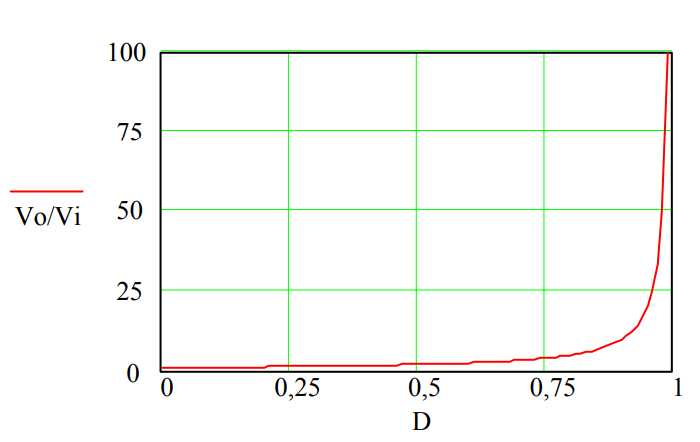
\includegraphics[scale=0.55]{imagens/grafico2_boost.png}
\caption{Relação entre o ganho estático e a razão cíclica em um conversor Boost.}\label{g2bo} 
\caption*{Fonte: Introdução aos conversores CC-CC (2001)}
\end{figure}

O comportamento da tensão e da corrente nos componentes do conversor Boost é ilustrada na figura \ref{g3bo}.

\begin{figure}[h]
\center
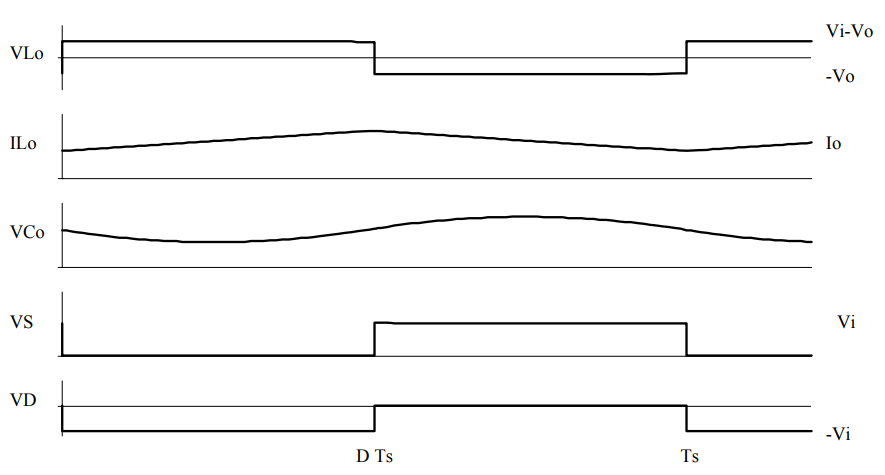
\includegraphics[scale=0.55]{imagens/grafico3_boost.png}
\caption{Tensão e corrente nos componentes do conversor Boost.}\label{g3bo} 
\caption*{Fonte: Introdução aos conversores CC-CC (2001)}
\end{figure}

As principais características do conversor Boost são sua capacidade de aumentar a tensão da saída, apesar de fornecer corrente de forma descontínua, e baixa distorção da corrente consumida da alimentação.


 
\subsubsection{Conversores Buck-Boost}

Resultado da combinação dos dois conversores que dão nome a este, o conversor Buck-Boost consegue elevar e abaixar a tensão. A figura \ref{cbobu} ilustra um circuito simplificado para esse conversor.

\begin{figure}[h]
\center
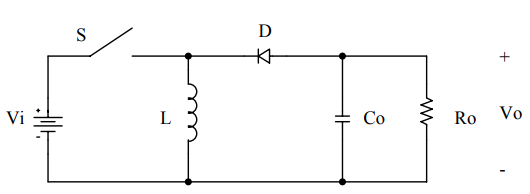
\includegraphics[scale=0.55]{imagens/circuito_buck_boost.png}
\caption{Circuito do conversor Buck-Boost.}\label{cbobu} 
\caption*{Fonte: Introdução aos conversores CC-CC (2001)}
\end{figure}

Durante a etapa de condução da chave $S$, a fonte fornece energia para o indutor $L$, enquanto o capacitor $C_o$ descarrega sobre o resistor $R_o$. Após a abertura da chave $S$, o indutor alimenta tanto o capacitor quanto a resistência, mas de forma invertida à fonte. A figura \ref{g1bobu} ilustra a tensão no indutor $L$.

\begin{figure}[h]
\center
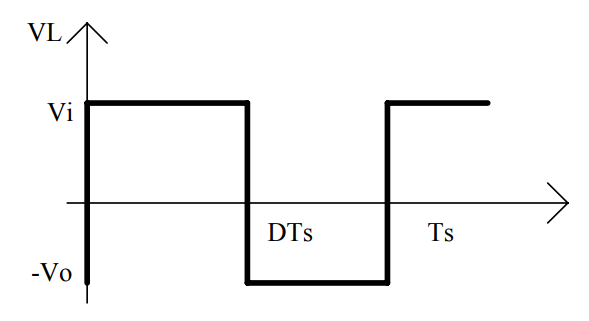
\includegraphics[scale=0.55]{imagens/grafico1_buck_boost.png}
\caption{Comportamento da tensão no indutor $L$ de um conversor Buck-Boost.}\label{g1bobu} 
\caption*{Fonte: Introdução aos conversores CC-CC (2001)}
\end{figure}

Considerando a tensão média no indutor nula, segue que \[
    \frac{1}{T_{s}}\int_{o}^{DT_{s}}V_{i}dt =  \frac{1}{T_{s}}\int_{o}^{(1-D)T_{s}}(V_{o} - V_{i})dt
\] \[
\implies\frac{V{o}}{V{i}} = \frac{D}{1-D}
.\] Logo, é fácil ver que o conversor pode tanto abaixar quanto elevar a tensão de forma contínua a partir da razão cíclica. A figura \ref{g2bobu} ilustra essa relação.

\begin{figure}[h]
\center
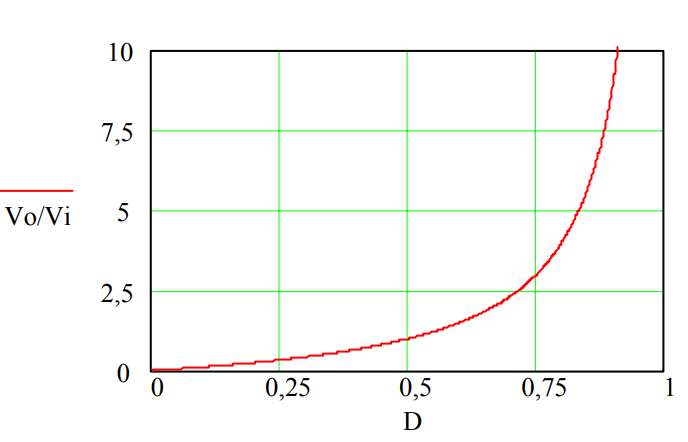
\includegraphics[scale=0.55]{imagens/grafico2_buck_boost.png}
\caption{Relação entre o ganho estático de um conversor Buck-Boost e a razão cíclica do chaveamento.}\label{g2bobu} 
\caption*{Fonte: Introdução aos conversores CC-CC (2001)}
\end{figure}

O comportamento da tensão e da corrente nos diversos componentes desse conversor está ilustrado na figura \ref{g2bobu}.

\begin{figure}[h]
\center
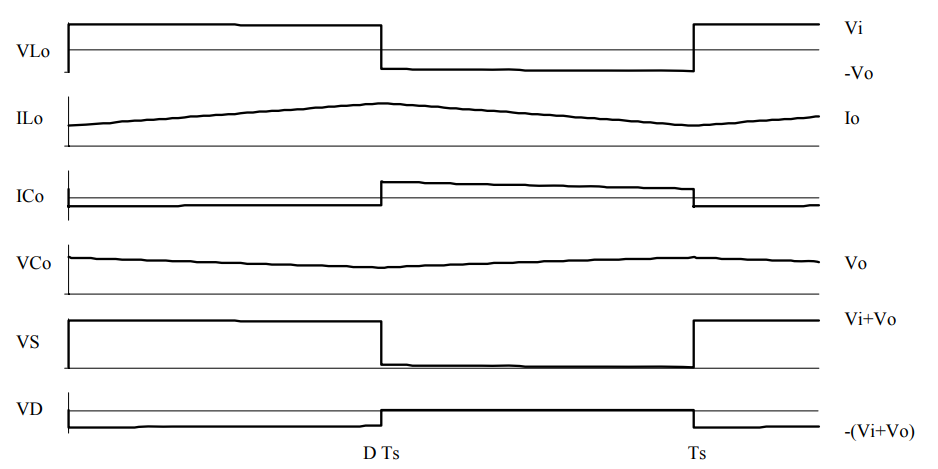
\includegraphics[scale=0.55]{imagens/grafico3_buck_boost.png}
\caption{Comportamento da tensão e da corrente nos diversos componentes de um conversor Buck-Boost.}\label{g3bobu} 
\caption*{Fonte: Introdução aos conversores CC-CC (2001)}
\end{figure}

Dessa forma, o conversor Buck-Boost fornece uma implementação que abaixa e eleva a tensão de forma contínua, mas distorce a corrente tanto para a alimentação quanto para a carga.


 
\subsection{Conversores CC-CA}

Também conhecidos como inversores, possuem como principal função transformar uma fonte contínua de alimentação em uma fonte alternada, simétrico, de frequência constante e tensão média nula. Conversores CC-CA podem ser categorizados ainda quanto à fonte utilizada, o número de fases e o número de fontes de alimentação.

Se o inversor opera em um fonte de corrente ele é chamado CSI (\emph{Current-Source Inverter}), enquanto que se opera em uma fonte de tensão é denominado VSI (\emph{Voltage-Source Inverter}), sendo essa última a mais comum.

Quanto ao número de fases, não há uma limitação clara, sendo dependente da aplicação, ainda que o mais comum seja vermos inversores monofásicos e trifásicos.

Por último, um inversor pode se beneficiar de múltiplas fontes de alimentação como uma forma de, dependo do arranjo, dispor de vários níveis de tensão. Por isso são chamados multiníveis.

Esse tipo de inversor tem ampla utilização na industria principalmente pois permitem o controle de velocidade para motores síncronos e de indução. Além disso, são também costumeiramente utilizados como fontes de alimentação para diversos sistemas trifásicos que se alimentam de alta tensão, uma vez que faz o intermédio entre fontes contínuas de alta tensão (e.g., transmissão HVDC) e cargas de corrente alternada.

Destaca-se que os transistores utilizados são assumidos bem dimensionados e serão tratados como chaves ideais.

\subsubsection{Inversores Monofásicos}

Dois arranjos serão estudados para o inversor monofásico: em semi-ponte e em ponte completa. Ambos podem ser observados na figura \ref{c1im}.

\begin{figure}[h]
\center
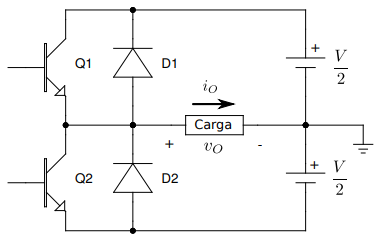
\includegraphics[scale=0.55]{imagens/circuito1_inversor_mono.png}
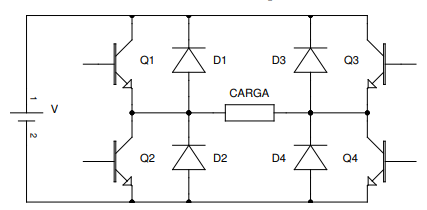
\includegraphics[scale=0.55]{imagens/circuito2_inversor_mono.png}
\caption{Circuitos de um inversor monofásico em semi-ponte. À esquerda, em semi-ponte;  direita em ponte completa.}\label{c1im} 
\caption*{Fonte: Apostila de eletrônica de potência (2015)}
\end{figure}

No caso da implementação em semi-ponte, através do chaveamento dos transistores Q1 e Q2 pode-se controlar a tensão observada pela carga. A figura \ref{g1im} ilustra esse comportamento. Não é difícil ver que se o controle de Q2 é replicado em Q3 e o de Q1 em Q4, temos o mesmo resultado, para a carga, no caso da implementação em ponte completa mas com amplitude dobrada. Nota-se que a tensão percebida pela carga é uma onda quadrada, mas simétrica e com frequência constante, desde que a frequência de chaveamento o seja.

\begin{figure}[h]
\center
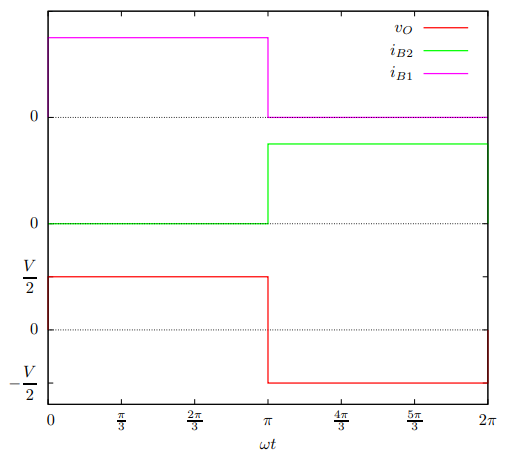
\includegraphics[scale=0.55]{imagens/grafico1_inversor_mono.png}
\caption{Tensão sobre a carga de um inversor monofásico em semi-ponte e correntes de acionamento dos transístores Q1 e Q2.}\label{g1im} 
\caption*{Fonte: Apostila de eletrônica de potência (2015)}
\end{figure}

Podemos, então, modelar a tensão de saída do inversor através da expansão em série de Fourier da onda quadrada gerada, i.e., \[
    v_{o} = \sum_{k=1}^{\infty}\frac{4A}{\left( 2k +1 \right) \pi}\sin{\left( 2k+1 \right) \omega{t}} 
,\] onde $A$ é a amplitude da tensão de saída (portanto $A = \frac{V}{2}$ para o inversor em semi-ponte e $A = V$ para o inversor em ponte completa), $\omega = 2\pi f$ é a frequência da tensão de saída.

Caso a carga seja puramente resistiva é evidente que a corrente possuirá o mesmo comportamento da tensão. No caso de uma carga com componente indutivo, a corrente na carga torna-se \[
    i_{o} = \sum_{k=1}^{\infty}\frac{4A}{\left( 2k+1 \right) \pi{|Z_{k}|}}\sin(\left( 2k+1 \right)\omega{t} - \phi_{k})
,\] onde $\tau = \frac{L}{R}$, $|Z_k| = \sqrt{R^{2} + (\left( 2k+1 \right) \omega{L})^2}$ e \[
\phi_{k} = \tan^{-1} \frac{\left( 2k+1 \right) \omega{L}}{R}
.\] 

Também pode-se escrever a corrente em função da amplitude $A$, de forma \[
i_o = \begin{cases}
    \frac{A}{R}(1-e^{-t/\tau}) &, t \in [0,\frac{T}{2}) \\
    \frac{-A}{R}(1-e^{-(t-\frac{T}{2})/\tau}) + I_{max}e^{-(t-\frac{T}{2})/\tau} &, t \in [\frac{T}{2},T)
\end{cases}
,\] onde: \[
    I_{MAX} = \frac{A}{R} \left(  \frac{1-e^{-\frac{T}{2\tau}}}{1+e^{-\frac{T}{2\tau}}}\right) 
.\]

Caso seja uma carga com componente capacitivo, a corrente pode ser descrita por \[
i_o = \begin{cases}
    I_{MAX}e^{-t/\tau} &, t \in \left[0,\frac{T}{2}\right) \\
    I_{MAX}e^{-(t-\frac{T}{2})/\tau} &, t \in \left[\frac{T}{2}, T\right)
\end{cases}
\] e a tensão \[
i_o = \begin{cases}
    A(1-e^{-t/\tau}) - V_{CO}e^{-t/\tau} &, t \in \left[0,\frac{T}{2}\right) \\
    A(1-e^{-(t-\frac{T}{2})/\tau}) + V_{C0}e^{-(t-\frac{T}{2})/\tau} &, t \in \left[\frac{T}{2}, T\right)
\end{cases}
,\] onde \[
    V_{C0} = A\frac{1-e^{-\frac{T}{2\tau}}}{1+e^{-\frac{T}{2\tau}}}
\] e \[
    I_{MAX} = \frac{A + V_{co}}{R}
.\]

A figura \ref{g3im} ilustra o comportamento da tensão e da corrente para ambas as cargas não lineares.

\begin{figure}[h]
\center
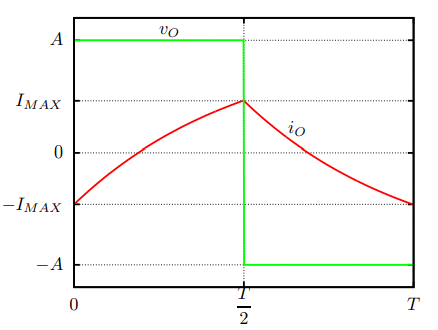
\includegraphics[scale=0.55]{imagens/grafico3_inversor_mono.png}
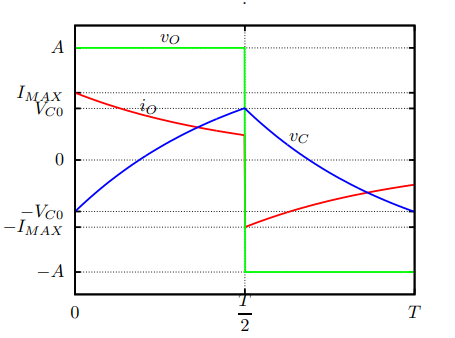
\includegraphics[scale=0.55]{imagens/grafico4_inversor_mono.png}
\caption{Corrente e tensão na carga de um inversor monofásico. À esquerda, carga RL; à direita, carga RC.}\label{g3im} 
\caption*{Fonte: Apostila de eletrônica de potência (2015)}
\end{figure}


 
\subsubsection{Inversores Trifásicos}


O circuito característico de um inversor trifásico pode ser ilustrado como na figura \ref{c1it}.

\begin{figure}[h]
\center
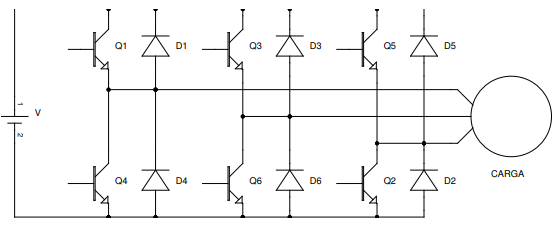
\includegraphics[scale=0.55]{imagens/circuito1_inversor_tri.png}
\caption{Estrutura básica de um inversor trifásico}\label{c1it} 
\caption*{Fonte: Apostila de eletrônica de potência (2015)}
\end{figure}

Serão estudadas duas formas de comutação simples para esse tipo de inversor. A primeira, chamada de comutação seis-pulsos 180º, consiste em acionar cada um dos 6 transistores durante meio ciclo (daí os 180º) igualmente espaçados. O acionamento dos transistores encontra-se ilustrado na figura \ref{g1it}, junto do resultado para a carga em termos de tensão de fase e linha. Veja que a tensão de linha (eficaz) nesse modo de operação é \[
V_R = \sqrt{\frac{2}{3}} V
.\] 

\begin{figure}[h]
\center
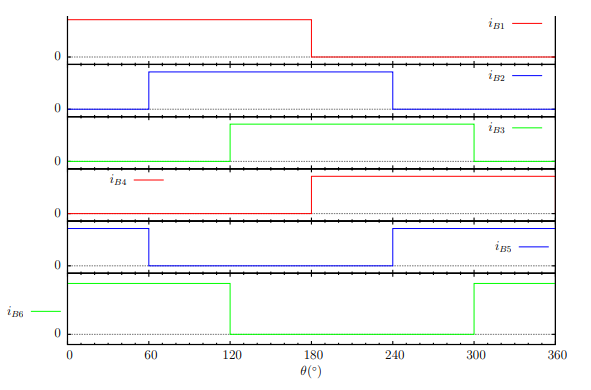
\includegraphics[width=0.32\textwidth]{imagens/grafico1_inversor_tri.png}
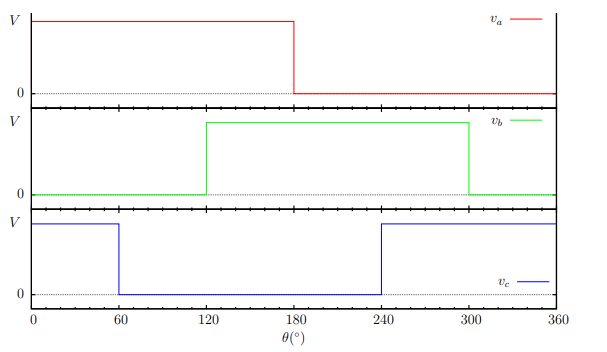
\includegraphics[width=0.32\textwidth]{imagens/grafico2_inversor_tri.png}
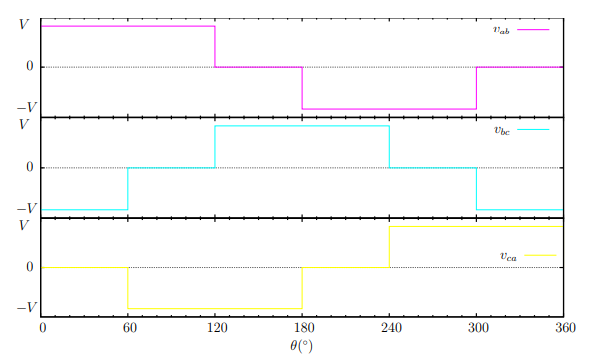
\includegraphics[width=0.32\textwidth]{imagens/grafico3_inversor_tri.png}
\caption{Acionamento dos transistores (à esquerda) da ponte inversora trifásica em operação seis pulsos 180º, assim como a tensão de fase (ao centro) e de linha (à direita) para a carga.}\label{g1it} 
\caption*{Fonte: Apostila de eletrônica de potência (2015)}
\end{figure}

Já o modo de comutação seis-pulsos 120º modifica o período de ativação de cada transistor para $\frac{2}{3}$ do período desejado, gerando intervalos de tensão não determinada, como pode ser visto na figura \ref{g4it}, estando os transistores em estado de alta impedância.
 
\begin{figure}[h]
\center
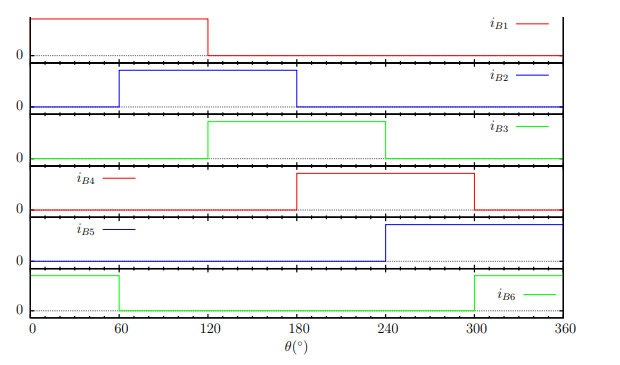
\includegraphics[width=0.32\textwidth]{imagens/grafico4_inversor_tri.png}
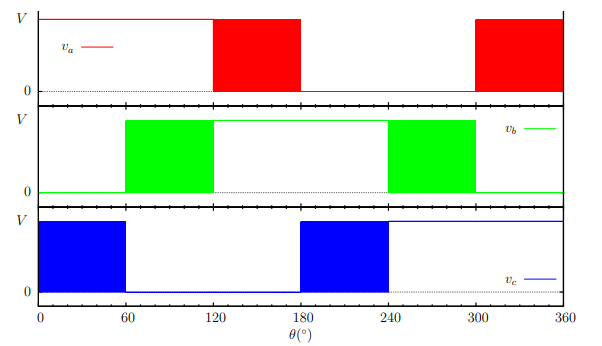
\includegraphics[width=0.32\textwidth]{imagens/grafico5_inversor_tri.png}
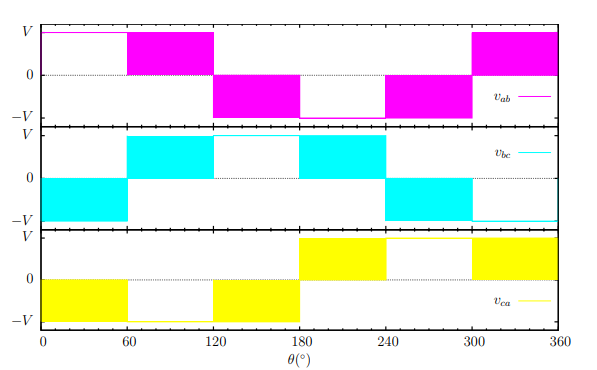
\includegraphics[width=0.32\textwidth]{imagens/grafico6_inversor_tri.png}
\caption{Acionamento dos transistores (à esquerda) da ponte inversora trifásica em operação seis pulsos 120º, assim como a tensão de fase (ao centro) e de linha (à direita) para a carga. Regiões sólidas representam um valor não determinado pelo inversor.}\label{g4it} 
\caption*{Fonte: Apostila de eletrônica de potência (2015)}
\end{figure}

Caso a carga seja puramente resistiva, a tensão aparente para essa será como ilustrado na figura \ref{g7it}. A tensão de linha (eficaz), então, torna-se \[
V_R = \frac{\sqrt{2} }{2}V
.\] 

 \begin{figure}[h]
\center
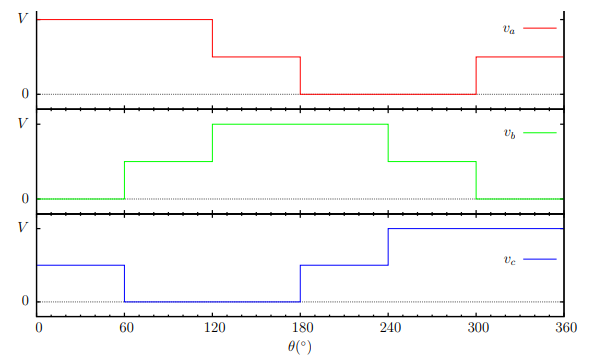
\includegraphics[width=0.45\textwidth]{imagens/grafico7_inversor_tri.png}
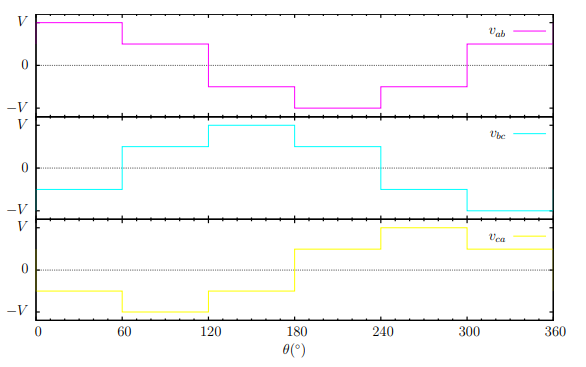
\includegraphics[width=0.45\textwidth]{imagens/grafico8_inversor_tri.png}
\caption{Tensão de fase (à esquerda) e linha (à direita) para uma carga resistiva em um inversor trifásico em modo de comutação seis-pontos 120º.}\label{g7it} 
\caption*{Fonte: Apostila de eletrônica de potência (2015)}
\end{figure}



